\documentclass[a4paper, 12pt]{article}

\usepackage{listings}
\usepackage{color}

\definecolor{dkgreen}{rgb}{0,0.6,0}
\definecolor{gray}{rgb}{0.5,0.5,0.5}
\definecolor{mauve}{rgb}{0.58,0,0.82}

\lstset{frame=tb,
	language=C,
	aboveskip=3mm,
	belowskip=3mm,
	showstringspaces=false,
	columns=flexible,
	basicstyle={\small\ttfamily},
	numbers=none,
	numberstyle=\tiny\color{gray},
	keywordstyle=\color{blue},
	commentstyle=\color{dkgreen},
	stringstyle=\color{mauve},
	breaklines=true,
	breakatwhitespace=true,
	tabsize=3
}

\usepackage[english]{babel}
\usepackage{microtype}
\usepackage{graphicx}
\usepackage{amsmath}
\usepackage{index}

\makeindex

\begin{document}
	\title{Tutorat microprocesseur}
	\author{Corentin GIELEN, Florian DERLIQUE, Miaoqi WANG, Maxence NEUS}
	\maketitle
	
	\newpage
	\tableofcontents
	\newpage
	
	\section{Introducion}
		Nous avons à réaliser un radar de contrôle routier.
		Le radar doit pouvoir réaliser les fonctions suivantes :
		\begin{enumerate}
			\item Mesurer la vitesse d'un véhicule qui entre dans sa zone d'action
			\item Permettre de changer la vitesse maximale authorisée à l'aide d'un clavier
			\item Si la vitesse mesurée est supérieure à la vitesse maximale, activer le flash et envoyer la vitesse mesurée sur l'imprimante série
		\end{enumerate}
	
		On nous demande ici en plus, de ne flasher que lorsque le vehicule se trouve à une distance de moins de 30m du radar afin que l'appareil photo puisse avoir une bonne vue de la plaque d'immatriculation.\\
		Malheureusement cette restriction nous amène à des limitations dans notre capacité à mesurer certaines vitesses mais ce point sera développé plus emplement plus loin.
		
	\newpage
	\section{Architecture Matérielle}
		\subsection{Matériel}
		Nous avons à notre dispositon les éléments suivants :
		\begin{itemize}
			\item Un télémetre qui fournit un signal analogique proportionnel à la distance entre le radar et la voiture
			qui donne une valeur entre 0V pour une distance de 0m et 5v pour une distance de 100m
			\item Un détecteur de présence qui passe de l'état 0 à l'état 1 lorsqu'une voiture entre dans le champ de mesure du télémetre
			\item Un flash que l'on peut déclancher directement sur un pin digital
			\item Une imprimante série pour imprimer les vitesses mesurées
			\item Les composants standards
		\end{itemize}	
		\subsection{Mise en place de l'architecture}
		\begin{figure}[h]
		\centering
		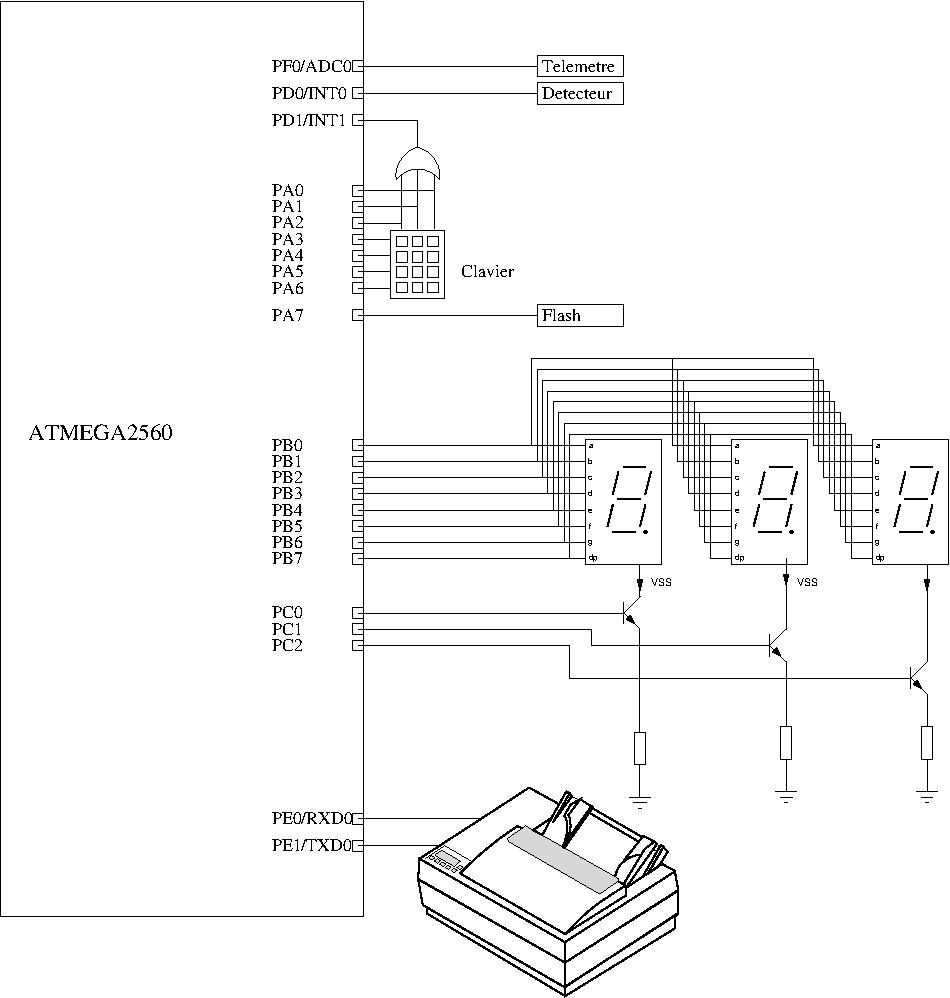
\includegraphics[width = 9cm]{schema.jpg}
		\caption{schema de cablage}
		\end{figure}
		\newpage
		\subsubsection{Interface utilisateur}
		Pour réaliser la fonction 2, nous avons besoin de permettre à l'utilisateur de rentrer une nouvelle valeur pour la vitesse maximale authorisée. Pour ce faire, nous avons incorporer un clavier 12 touches (0-9, Valider, Annuler) et 3 afficheurs 7 segments multiplexés pour afficher la valeur entrée à l'utilisateur.\\
		Le clavier est branché sur les pins PA[0:6] avec une porte OU qui permettra par la broche PD1/INT1 de travailler par interruption pour la lecture du clavier.\\
		Pour ce qui est des afficheurs 7 segments, ils sont reliés au port B pour la valeur à afficher et multiplexé par les pins PC[0:2] qui font la conection des bases des afficheurs à la masse via des transistors et des résistances de tirage.
		\subsubsection{Appareils de mesure}
		Comme le Télémetre nous fournis une valeur analogique, nous avons choisis de le relier à la broche PF0/ADC0 pour pouvoir réaliser une conversion dessus.\\
		Nous avons choisis d'utiliser le détecteur de présence par intéruption, nous le relions donc à la broche PD0/INT0.\\
		\subsubsection{Sorties utilisateur}
		Pour le flash, nous l'avons relié à la dernière broche inutilisée du port A, PA7, nous supposons qu'un appareil photo déclanchable par un front montant est relié à la même broche pour pouvoir prendre une photo de l'automobiliste qui est en exces de vitesse.\\
		L'impimante série est reliée à l'interface USART0 (PE0/RXD0;PE1/TXD1), L'imprimante fonctionne à 1200 bauds, 8bits de message, 1 bit stop et pas de parité, son initialisation sera développée dans la section 3.\\
	\newpage
	\section{Architecture Code}
		\subsection{Initialisation}
		Le convertisseur analogique numérique (ADC) est mis en place de sorte qu'il réalise des convertions sur demande en lisant sur la broche PF0/ADC0 en envoyant une interuption à la fin de la convertion.
		\begin{lstlisting}
			//ADC (convertion ADC0, single convertion)
			ADMUX = 0b0010 0000
			ADCSRA = 0b1000 1111
			ADCSRB = 0x00
		\end{lstlisting}
		
		Nous utiliserons un WatchDog pour temporiser nos mesures, celui çi est ici reglé pour envoyer des interuptions toute les 0.5s (Ce choix est discuté dans la partie limites).
		\begin{lstlisting}
			//Watchdog (interruptions toute les 0.5s)
			WDTCSR = 0x10 // enable change
			WDTCSR = 0b0101 0101
		\end{lstlisting}

		Pour envoyer les mesures à l'imprimante nous devons utiliser la liaison série de l'ATMEGA comme décrit en 2.2.3, nous avons caculé la valeur de UBRR grâce à la formule donné dans la documentation $UBRR = \dfrac{f_{osc}}{16*BAUD} - 1$ qui nous donne UBRR = 832, soit 0x340 à répartir sur les registres UBRRL0 et UBRRH0.
		\begin{lstlisting}
			//printer (envoi uniquement, pas de verification, conforme au CDCF)
			UBRR (f = 16MHz) = 832
			UBRRH0 = 0x03
			UBRRL0 = 0x40
			
			UCSR0A = 0x00
			UCSR0B = 0b0000 1000
			UCSR0C = 0b0000 0110			
		\end{lstlisting}	
	
		On règle ici les afficheurs et le clavier comme décrit en 2.2.1.
		\begin{lstlisting}
			//Clavier et afficheurs
			DDRA = 0b0001 1111
			DDRB = 0x0111 1111
			DDRC = 0b0000 0111
		\end{lstlisting}
		\newpage
		On reprends ici les différents vecteurs d'interruptions utilisés ainsi que les noms des subsoutines associées.
		\begin{lstlisting}
			//vecteurs d'interuption
			.org 0x0002
				JMP IRQ_detecteur
			.org 0x0004
				JMP IRQ_clavier
			.org 0x0018
				JMP IRQ_Watchdog
			.org 0x003A
				JMP IRQ_convertion
		\end{lstlisting}
		\subsection{Structure globale}
		Afin de réaliser les mesures de vitesses, nous n'avons à notre disposition que la position du vehicule, nous allons donc avoir besoin de mesurer la distance entre le radar et le vehicule à un intervale régulier pour pouvoir par la suite calculer la vitesse. \\
		Le processus de mesure commence lorsque le vehicule entre dans la zone de mesure du télémetre et que le détecteur de présence envoie un signal d'interruption qui amène à l'appel de la procédure d'interruption $IRQ\_detecteur$.
		
		\begin{lstlisting}
			// detection d'une voiture par le detecteur de presence  
			IRQ_Detecteur:
				si cpt_detection==0 alors saut init_watch // si le capteur est en front montant on initialise le WatchDog
				//si non on reinitialise le WatchDog 
				WDTCSR<-0b00010000
				WDTCSR<-0b00000000
				cpt_detection <- 0 
				RETI
				init_watch: 
					WDTCSR<-0b00010000
					WDTCSR<-0b01001101
					cpt_detection=1
				RETI
		\end{lstlisting}
		Cette procédure a pour but de démarrer ou d'arreter le WatchDog selon si le vehicule qui a été détecté entrait ou sortait de la zone de mesure (l'interuption est règlée pour être déclanchée sur front montant comme déscendant), cette distinction est faite grâce à une variable $cpt\_detection$ qui est mise à 1 lorsqu'un vehicule est présent dans la zone et à 0 lorsque ce n'est plus le cas.\\
		
		Par la suite, le WatchDog va maintenant déclancher des interuptions toute les 0.5s comme defini lors de l'initialisation. voyons maintenant ce que fait cette procédure:\\
		
		\begin{lstlisting}
			//interuption du watch_dog
			// quand le watch_dog est activer on active la prise de mesure
			IRQ_WDT :
				ADCSRA<-0b11001111
				RETI
		\end{lstlisting}
		Ici tout ce que fait la procédure c'est lancer une convertion sur ADC0 afin de mesurer la distance du radar au vehicule, lorsque cette mesure sera faite, le convertisseur analogique numérique lancera une interruption qui déclanchera la procédure $IRQ\_convertion$.\\
		
		\begin{lstlisting}
			IRQ_CONVERTION:
			mesure <- ADC
			si(cpt_mesure) == 0 alors saut cpt0 // c'est a dire c'est la premiere mesure de vitesse 
			si(cpt_mesure) == 1 alors saut cpt1 // c'est la 2 eme mesure de vitesse
			
			cpt0:
			Pos1<-mesure //  alors on stocke la valeur mesure par la conversion entre 0 et 255
			cpt_mesure <- 1 
			RETI
			
			cpt1:
			pos2<-mesure
			if(Pos1-Pos2)>vitesse_limite saut distflash // si la vitesse et superieur a la limite et que la voiture est a plus de 30m du tel
			cpt_mesure <- 0
			RETI
			
			distflash:// si la vitesse est superieur on attends que la distance au radar soit inferieur a 30m
			posflash<-76// 76 en annalogique soit 255/100*30 pour avoir les 30m
			si posflash<76 alors saut port_serie 
			ADCSRA<-0b11001111
			
			port_serie:
			call flash 
			call imprime 
			RETI
		\end{lstlisting}
		Ici la mesure de distance est stockée dans un buffer qui correspond à la première ou à la seconde mesure pour pouvoir par la suite faire la difference entre les deux position et ainsi obtenir la vitesse que l'on cherche à mesurer. On compare ensuite la valeur mesurée avec la vitesse maximale autorisée qui a été entrée et si elle est atteinte et que la dernière mesure de position était inferieure à 30m, on lance la procédure de flash et d'envoi de la vitesse mesurée à l'imprimante.\\
		Cette vitesse est d'abord convertie en $km/h$ à partir de la mesure en $m/s$ qui est utilisée en interne et ensuite envoyée caractère par caractère à l'imprimante. 
		
		
\end{document}